\section{General Terms and Notations}

Before MMIX is described in further detail, a few terms and notations that are used throughout this thesis should be introduced.

At first, numbers without any prefix or other qualification should be read in decimal base, whereas numbers prefixed with '\haddr{}' should be read in hexadecimal base. General purpose registers are named \dr{X}, where `X` is between 0 and 255. Special registers are named \sr{X}, where `X` is any of `A`, `B`, \dots, `Z`, `BB`, `TT`, `WW`, `XX`, `YY`, `ZZ`. The quantities in MMIX are:
\begin{table}[H]
	\begin{tabular}{| p{13mm} | p{13mm} | p{105mm} |}
		\hline \textbf{Name} & \textbf{Bits} & \textbf{Unsigned and signed integer range} \\
		\hline Byte & 8 &
		$0 \dots 255$ \newline
		$-128 \dots 127$
		\\
		\hline Wyde & 16 &
		$0 \dots 65535$ \newline
		$-32768 \dots 32767$
		\\
		\hline Tetra & 32 &
		$0 \dots 4,294,967,295$ \newline
		$-2,147,483,648 \dots 2,147,483,647$
		\\
		\hline Octa & 64 &
		$0 \dots 18,446,744,073,709,551,615$ \newline
		$-9,223,372,036,854,775,808 \dots 9,223,372,036,854,775,807$
		\\
		\hline
	\end{tabular}
	\caption{Quantities in MMIX \citep[pg. 3]{mmix-doc}}
\end{table}

The virtual memory is an array called M. An access of $2^t$ consecutive bytes at location $k$ is written as \vmem{2^t}{k}, where $k$ is $2^t$-byte aligned (the least significant $t$ bits are zero). That means, for example \vmemh{1}{1234} denotes the byte at location \haddr{1234} and \vmemh{8}{100} the octabyte at location \haddr{100}. The virtual memory is divided in two halfs. The memory space \haddro{0000}{0000}{0000}{0000} \dots \haddro{7FFF}{FFFF}{FFFF}{FFFF} is called \i{user space} and \haddro{8000}{0000}{0000}{0000} \dots \haddro{FFFF}{FFFF}{FFFF}{FFFF} is called \i{privileged space}. Furthermore, the location of the \glslink{PC}{instruction pointer}, called \i{@}, determines the mode in which MMIX operates. If it is in user space, it is in \i{user mode}, otherwise in \i{privileged mode}. Finally, MMIX distinguishes between \i{arithmetic exceptions} (\glslink{Exception}{AE}) like division by zero or integer overflow, which are handled by the user application, \i{program exceptions} (\glslink{Exception}{PE}) such as privileged instruction or protection fault, which are handled by the operating system, and \i{machine exceptions} (\glslink{Exception}{ME}) like power failure, which are as well handled by the OS.

\section{Instruction Format}

Each MMIX instruction is described by a tetra, which consists of four parts:\\
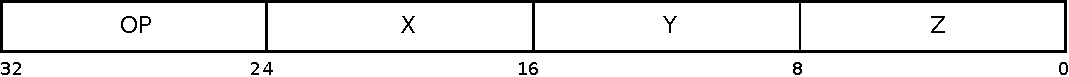
\includegraphics[width=\linewidth]{img/instruction-crop.pdf}

The first byte is the \i{opcode} of the instruction and the other three bytes specify the \i{operands}. Thus, MMIX allows (and uses) 256 instructions with 3 operands, each having 256 possible values. The typical instruction has the meaning "Set register {\tt X} to the result of {\tt Y} OP {\tt Z}". \citep[pg. 2]{mmix-doc}

In this thesis, all instructions are at first outlined with a box that contains the mnemonic, the operands of the instruction and the its effect. Afterwards the instruction is illustrated in further detail -- including special cases and raised \glslink{Exception}{AEs} or \glslink{Exception}{PEs}. The box looks like the following:
\instrtbl
	{\mi{ADD|SUB \$X,\$Y,\$Z|Z}}
	{$\dr{X} \leftarrow s(\dr{Y}) +|- \sdrimm{Z}$}

\noindent This describes the four instructions \mi{ADD}, \mi{ADDI}, \mi{SUB} and \mi{SUBI}. As in this example, many MMIX instructions come in two forms: In the first one, the {\tt Z}-operand is a register, in the second one it is an \glslink{Immediate Value}{immediate value}. Since there is no other difference, these are handled at once by saying "\udrim{Z}". Furthermore, \mi{ADD} and \mi{SUB} are very similar, so that they are grouped together. The notation $s(...)$ denotes, that MMIX interprets it as signed and uses two's complement arithmetic. Otherwise it means that MMIX treats the value as unsigned. Thus, the effect in the box shown above can be read as
\begin{itemize}
	\item \mi{ADD} sets \dr{X} to the result of the addition of \dr{Y} and \dr{Z}, interpreting both as signed values and hence, using signed arithmetic,
	\item \mi{ADDI} sets \dr{X} to the result of the addition of the signed value \dr{Y} and unsigned \glslink{Immediate Value}{immediate value} {\tt Z},
	\item \mi{SUB} sets \dr{X} to the result of the substraction of the signed value \dr{Y} and signed value \dr{Z} and
	\item \mi{SUBI} sets \dr{X} to the result of the substraction of the signed value \dr{Y} and unsigned \glslink{Immediate Value}{immediate value} {\tt Z}.
\end{itemize}
\glslink{Immediate Value}{Immediate values} are always interpreted unsigned in MMIX. Additionally, if one of the operands {\tt X}, {\tt Y} and {\tt Z} is not mentioned in the name, it means implicitly that the corresponding byte has to be zero. If it is not, MMIX will raise a \i{breaks rules} \glslink{Exception}{PE}.

Although the effects description will be straight forward for most of the instructions, it is not meant to be always complete or self-explaining, because that would be too verbose and would require a formal language definition for some instructions. Rather, it should be seen as a quick overview of what the instruction does. Thus, if necessary, the text below the box will clarify the effects description or adds further information.

